%%%%%%%%%%%%%%%%%%%%% chapter.tex %%%%%%%%%%%%%%%%%%%%%%%%%%%%%%%%%
%% At the end, it won't supposed to have
%% %! For Obs
%% %R For bib
%%%%%%%%%%%%%%%%%%%%%%%% Springer-Verlag %%%%%%%%%%%%%%%%%%%%%%%%%% 
%\motto{Use the template \emph{chapter.tex} to style the various elements of your chapter content.}
\chapter{Herramientas libres para construir proyectos Hardware-Software}
\label{intro} % Always give a unique label
%

\begin{svgraybox}
\abstract{En los anteriores cap�tulos se ha tratado el uso de herramientas libres generar tanto los archivos finales a implementar en tanto para dise�os software como para dise�os Hardware. En este cap�tulo se pretende mostrar las diferentes etapas de la construcci�n de los dise�os Hardware/Software a partir de la herramienta Make y la cadena de compilaci�n basada en GCC.}
\end{svgraybox} 

\section{Introduccion}

Introduccion ....

\label{sec:1}

%%%%%%%%%%%%%%%%%%%%% %%%%%%%%%%% %%%%%%%%%%%%%%%%%%%%%%%%%%%%%%%%%
%
% This section is intended to provide a review on how to use the 
% the make to build pojects HW/SW
%
%%%%%%%%%%%%%%%%%%%%%%%% %%%%%%%%%%%%%%% %%%%%%%%%%%%%%%%%%%%%%%%%%
\section{Makefile}
%Para qu� se usa ....
%Implicaciones en el desarrollo de este libro
%El problema que los proyectos son muy extensos en c�digo y reconstruir todo es tedioso y repititivo....
s
El desarrollo de aplicaciones a partir de herramientas libres se apoya en la herramienta de construcci�n \textit{make}, la cual automatiza la creaci�n los archivos binarios de una aplicaci�n. La herramienta construcci�n \textit{make} comunmente llamada constructor, utiliza el archivo \textbf{Makefile} para tomar la especificaci�n del proyecto a construir. Con base en el \textit{Makefile} se ejecutan las reglas necesarias para construir el proyecto. En general el objetivo final del \textit{make} es construir una aplicaci�n, pero dada la flexibilidad que tiene se utiliza para construir cualquier tipo de proyecto que requiera muchas etapas de compilaci�n.

\subsection{Target, prerequisitos y reglas asociadas}

El constructor a trav�s de las reglas descritas en el archivo \textit{Makefile} determina cual y cuando se debe reconstruir un archivo para completar la construcci�n del proyecto completo; todo esto se realiza  en base a las marcas de tiempo de los archivos fuentes y el de salida (\textit{target}). S� los archivos fuentes que son prerequisitos de una regla tiene una marca de tiempo m�s reciente, el constructor determina que este archivo se debe reconstruir.\\

Las reglas del constructor se componen de un \textit{target} o archivo de salida (generalmente un archivo de salida por regla) y una serie de pre-requisitos para cada regla. Los pre-requisitos de cada regla se deben encontrar en las rutas de b�squeda del constructor para completar la construcci�n del proyecto; s� alg�n pre-rerquisito no existe el construcctor buscar� una regla asociada para su construci�n. Dado el caso que no exista alg�n archivo pre-requisito ni una regla asociada a este, el constructor falla con un mensaje de error de falta de pre-requisitos. A continuaci�n se muestra un ejemplo de la sintaxis de una regla para compilar \textit{foo.c} en \textit{foo.o}

\begin{lstlisting}
target1.o:	source1.c header1.h
			gcc -c source1.c
\end{lstlisting}

En las reglas del constructor, el nombre del archivo ubicado antes de los dos puntos (\textbf{:}) se le denomina \textit{target} en este caso \textit{target1.o}\textbf{:}. La lista de archivos que suceden a los dos puntos (\textbf{:}) se le llama la lista de prerequisitos.

Los pre-requisitos son los archivos que el \textit{target} necesita para su construcci�n, en este caso \textit{source1.c} y \textit{header1.h}. El tipo de archivo del \textit{target} y de los prerequisitos no tiene importancia dado que �nicamente se verifica su existenc�a y marca de tiempo. La l�nea que sigue al \textit{target} se le conoce como la primer linea de ejecuci�n de la regla o \textit{recipe}. Es necesario identar con un car�cter de tabulaci�n ($\rightarrow$) las lineas de comandos para que el constructor las ejecute correctamente. La ejecuci�n del \textit{recipe} se realiza en una consola diferente a la en que se invoca el comando \textit{make}. Cuando se tienen lineas muy extensas se puede usar el car�cter \textit{backslash} \textbf{\\}

\subsubsection{Tipos de reglas del constructor}

Existen diferentes tipos de reglas que el constructor puede tomar como referencia para ejecutar comandos externos. Estas reglas pueden ser reglas expl�citas, reglas basadas en comodines, reglas imperativas o reglas vac�as.

\paragraph{Reglas explicitas:} Las reglas expl�citas son las que constructor toma cuando un \textit{target} no se encuentra actualizado. El anterior ejemplo muestra como una regla explicita asociada al \textit{target1.o}. En algunas ocaciones dos o m�s \textit{targets} tienen los mismos prerequisitos para estos casos se pueden definir todos los \textit{targets} en una lista y asociarlos a una sola regla:

\begin{lstlisting}
target1.o target2.o:	source1.c header1.h
\end{lstlisting}

\paragraph{Reglas basadas en comodines \textit{Wildcards}:}

Cuando los proyectos contienen una gran cantidad de objetos por construir la craci�n de un \textit{Makefile} puede tornarse en una tarea repititiva y tomar un tiempo considerable. Para evitar esto el constructor tiene la herramienta de comodines (\textit{wildcards}), los comodines permiten agilizar la creaci�n de un \textit{Makefile} mediante la reducci�n de la cantidad de c�digos que deban construir. Dada la relaci�n estrecha entre el constructor y el \textit{shell} los comodines all� utilizados son heredados por el constructor, los comodines m�s utilizados son:
\begin{itemize}
	\item \textbf{\~}	:   Este s�mbolo se usa para representar la ruta de la carpeta \textit{home} del usuario que ejecuta el constructor.
	\item \textbf{*}	:   El aster�sco es usado para reemplazar una cadena de caracteres completa por ejemplo: Los siguientes archivos \textit{target1.o}, \textit{target2.o} y \textit{target3.o} se pueden representar como \textit{*.o}
	\item \textbf{?}	:   El funcionamiento de este car�cter es similar al \textbf{\*} pero en este caso no se remplaza una cadena completa sino un solo car�cter.
\end{itemize}

\paragraph{Reglas de ejecuci�n imperativa (.\textit{PHONY}):}

Generalmente las reglas incluidas en los \textit{Makefile} son reglas de tipo explicitas, como ya se mencion� estas reglas revisan la relaci�n entre el  \textit{target} y sus prerequisitos. Si se requiere que una regla se ejecute sin tomar en cuenta ninguna relaci�n de los prerequisitos y el \textit{target} se puede usar las reglas de tipo imperativa (.\textit{PHONY}). Un ejemplo claro de cuando se requiere utilizar las reglas imperativas en el caso de tener el siguiente \textit{Makefile}. Este archivo  tiene la regla \textit{clean} la cual no tiene prerequisitos y ejecuta el comando \textbf{rm -f *.o} para eleminar todos los archivos con extensi�n \textit{o}. La ejecuci�n de esta regla se puede realizar mediante  \textbf{\$ make clean}. 

\begin{lstlisting}
clean:
		rm -f *.o
\end{lstlisting}

La anterior regla se ejecuta sin ning�n inconveniente cuando no existe un archivo llamado \textit{clean} dentro de las rutas de b�squeda del cosntructor, dado que no tiene ning�n pre-requisito esta regla siempre se ejecuta al ser invocada. Pero si en la ruta del constructor existe un archivo de nombre \textit{clean} el constructor determina que el \textit{target} de dicha regla se encuentra al d�a y no se debe ejecutar sus comandos de construcci�n terminando su ejecuci�n con la siguiente salida:

\begin{lstlisting}
$ make clean
make: 'clean' is upt to date.
$
\end{lstlisting}

Para prevenir este comportamiento indeseado se puede declarar la regla de la siguiente manera:

\begin{lstlisting}
.PHONY: clean
clean:
		rm -f *.o
\end{lstlisting}

La regla \textit{.PHONY} fuerza la ejecuci�n de esta regla independientemente si el \textit{target} est� al d�a, todos los comandos de la regla se ejecutan cuando es invocada o es pre-requisito de otra regla en ejecuci�n.

Por otra parte existen reglas tipo \textit{PHONY} prestablecidas o est�ndares, estas reglas son definidas directamente por el constructor. Cada una de ellas se muestran en la siguiente tabla:


\begin{table}
\caption{Reglas imperativas comunes}
	\begin{tabular}{p{0.3\textwidth}p{0.7\textwidth}}
	
	\hline
	\textit{Target} & Funci�n (\textit{\$}) \\
	\hline
	
	\textbf{all} 		& 	Realiza todas las tareas necesarias para construir el proyecto \\
	\textbf{install} 	&	Instala la aplicaci�n tomando los binaros compilados \\
	\textbf{clean} 		&	Borra los binarios de la aplicaci�n y los archivos generados en su construcci�n \\
	\textbf{distclean} 	&	Borra todos los archivos generados que no hacen parte del codigo fuente de la distribuci�n \\
	
	
	\end{tabular}
\end{table}

\subsubsection{Reglas vaci�s}

Las reglas vacias son una variante directa de las reglas imperativas; estas reglas generalmente se usan para guardar un evento de construcci�n. La forma en que se puede guardar un evento de construcci�n es mediante la ejecuci�n del comando \textbf{touch} sobre el \textit{target}. 

\begin{lstlisting}
plot: source1.c header1.h
		touch plot
\end{lstlisting}

\subsection{Variables}

Las variables del constructor se utilizan para representar cadenas de caracteres, que pueden hacer referencia a nombres de archivos, directorios, opciones del compilador, programas a ejcutar en la construcci�n de la aplicaci�n, en general puede representar virutalmente cualquier cosa. Para definir una variable se debe ubicar el nombre de la variable en una nueva linea seguido del s�mbolo \textbf{=} y por �ltimo el valor que se desa contener. Para expandir la variable o usar su contenido se usa la misma sintaxis del \textit{bash} \$(\textit{(nombre-variable)})\\

El nombre de una variable no puede contener los carateres especiales \textbf{:}, \textbf{\#}, \textbf{\=} o espacios en blanco, por otra parte los nombres de las variables al igual que la variables del \textit{bash} son sensibles a mayusculas y minusculas. Se recomienda el uso de mayusculas sostenidas para las variables que sean par�metros de conficuraci�n, rutas del sistema y minusculas para el nombre de archivos de salida, programas que se deban ejecutar. 

\subsubsection{Variables autom�ticas}

Las variables autom�ticas permiten acceder a nombres preestablecidos de los componentes de una regla, como el \textit{target}, los prerequisitos. A continuaci�n se listan las variables autom�ticas m�s frecuentes:

\begin{table}
\caption{Variables autom�ticas}
	\begin{tabular}{p{0.1\textwidth}p{0.9\textwidth}}
	\hline
	\textit{Variable} & Funci�n  \\
	\hline

	\textbf{@} 		& Denota el nombre del \textit{target} de la regla.\\
	\textbf{\%}		& Denota el nombre del archivo dentro de una lista.\\
	\textbf{<}		& Es el nombre del primer prerequisito de la regla.\\
	\textbf{?}		& El nombre de todos los prerequisitos de la regla y que tienen una marca de tiempo mayor al \textit{target} en una lista separada poro espacios\\
	\textbf{\^}		& Es la lista de todos los prerequisitos de la regla separada por espacios. Los nombres repetidos son autom�ticamente eliminados para evitar ejecuciones reentrantes en el construcctor.\\
	\textbf{+}		& Es la lista de todos los prerequisitos de la regla separados por espacios, esta lista incluye nombres repetidos. \\
	\textbf{*}		& Es el nombre del archivo de salida sin su extensi�n de salida.
	\end{tabular}
\end{table}

La variables autom�ticas del constructor tambien se deben expandir al llamase es decir, al constructor se le debe decir que el caracter que se est� escribiendo es una variable, para eso se debe anteponer el caracter \textbf{\$} antes de cada variable autom�tica.

%\subsubsection{Variables autom�ticas de rutas de archivos (VPATH y vpath)}

%Cuando se tienen proyectos con gran cantidad de archivos usualmente los desarrolladores crean una estructura de carpetas organizando de esta manera el c�digo.



%%%%%%%%%%%%%%%%%%%%% %%%%%%%%%%% %%%%%%%%%%%%%%%%%%%%%%%%%%%%%%%%%
%
% This section is intended to provide a review on how to use the 
% GNU Toolchain and its parts to buil SW
%
%%%%%%%%%%%%%%%%%%%%%%%% %%%%%%%%%%%%%%% %%%%%%%%%%%%%%%%%%%%%%%%%%

\section{Herramientas compilaci�n y desarrollo de proyectos SW}%%%Esto est� feo.... Nombre m�s espec�fico

%!Esto necesita sustento en un libro falta incluir referencias de esta secci�n

%!Esto es solo una idea de introducci�n a la secci�n falta cambiar
Para el desarrollo de aplicaciones \textit{software} mediante lenguales de alto nivel perm�ten acelerar el desarrollo de la aplicaci�n, pero requiere de un conjunto de herramientas para la creaci�n del archivo final. Estas herramientas llevan el conjunto de archivos fuentes y paso a paso los convierten en un archivo ejecutable por la m�quina, llamado binario. 

%!Esta figura toca hacerla conteniendo las dos y explicarlas en el texto de abajo
\begin{figure}[h]
  \begin{center} 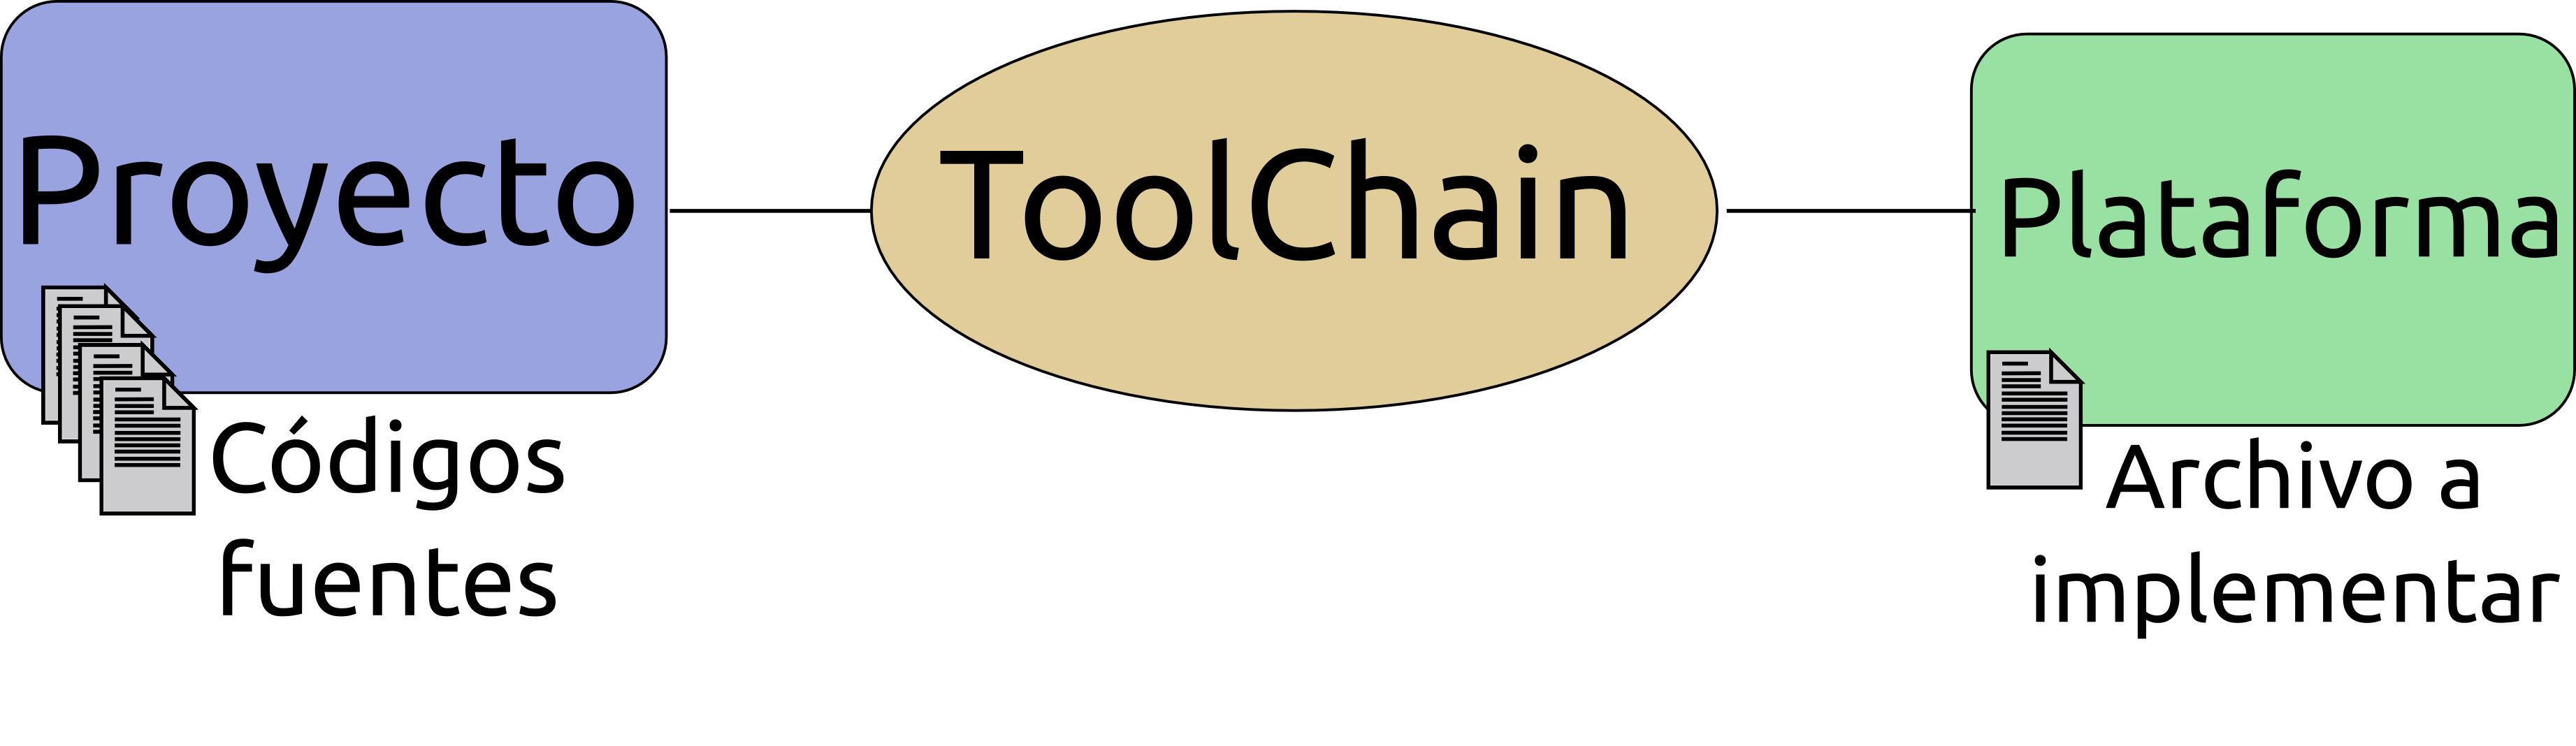
\includegraphics[scale=.5]{./anexo1/images/toolchain_reducido} \end{center}
  \caption{Flujo de dise�o SW utilizando la cadena de herramientas GNU}\label{toolchain_flow}
\end{figure}

\section{Flujo de dise�o software}
%R Real-Time Concepts for Embedded Systems
En la figura \ref{toolchain_flow} se ilustra la secuencia de pasos que se realizan desde la creaci�n de un archivo de texto que posee el c�digo fuente de una aplicaci�n hasta su implementaci�n en la tarjeta de desarrollo. Los pasos necesarios para generar un ejecutable para un sistema embebido son:

\begin{figure}[h]
  \begin{center} 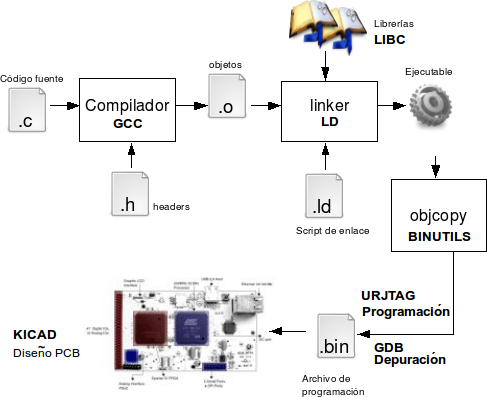
\includegraphics[scale=.6]{./anexo1/images/SW_design_flow} \end{center}
  \caption{Flujo de dise�o SW utilizando la cadena de herramientas GNU}\label{toolchain_flow}
\end{figure}

\begin{enumerate}
 \item \textbf{Escritura del c�digo fuente:} Los entornos de desarrollo \textit{software} IDE (\textit{integrated development environment}) proveen de un editor de texto y la colecci�n de herramientas est�n integradas en la misma aplicaci�n, para el caso de desarrollo de aplicaciones con \textit{software} libre existen alternativas como \url{www.eclipse.com} para la integraci�n de herramientas, pero no es un requisito para escribir c�digos fuentes el uso de un editor en particualar, cada programador puede escribir sus c�digos en la interfaz que le resulte m�s amigable. Los codigos fuentes de los programas para sistemas embebidos generalmente son escritos en C/C++. Algunas partes espec�ficas son escritas en lenguaje ensamblador por motivos de eficiencia en tiempo de ejecuci�n o tama�o. 

 \item \textbf{Compilaci�n:} Los archivos fuentes C y los archivos de ensamblador (generamente s) son tomados por las herramientas de compilaci�n para crear archivos tipo objetos. Estos objetos contienen las instrucciones que el procesador deber� ejecutar cuando las funciones sean invocadas para cumplir con la funcionalidad deseada. Adem�s, estos archivos contienen la informaci�n de las etiquetas usadas en el proceso de enlazado e informaci�n sobre la compilaci�n misma. Por �ltimo, los objetos no contienen las direcciones espec�ficas de donde se implementa una funci�n, por ejemplo, el compilador busca en los encabezados (\textit{headers} .h) de la funci�n \textit{printf} en la librerira \textit{stdio.h}, pero no busca el segmento de c�digo donde est� implementada.
%!!!Aqu� voy JRB-- Adecuando cosas!!!!!!!!!!!!!!!!!!!!!!!!!!!!!!!!!!!!!!!
 \item \textbf{Enlazado:} En esta etapa se realizan dos tareas: 
  \begin{enumerate} 
    \item Se enlazan los archivos tipo objeto del proyecto junto con las librer�as, si una determinada funci�n no es definida por ninguna de las librer�as pasadas como par�metro al enlazador (\textit{linker}), este generar� un error y no se generar� el ejecutable.
    \item Se definen la posiciones f�sicas de las secciones del ejecutable (tipo ELF), esto se realiza a trav�s de un \textit{script de enlazado} que define de forma expl�cita su localizaci�n.
  \end{enumerate}

 \item \textbf{Extracci�n del archivo de programaci�n} En algunas aplicaciones es necesario extraer �nicamente las secciones que residen en los medios de almacenamiento no vol�til y eliminar las dem�s secciones del ejecutable. Esto se realiza con la herramienta \textit{objcopy}, la cual, permite generar archivos en la mayor�a de los formatos soportados por los programadores de memorias y procesadores, como por ejemplo S19 e Intel Hex. Adicionalmente se puede generar un archivo binario que contiene las instrucciones en lenguaje del procesador, y pueden ser descargadas directamente a la memoria de la plataforma.

 \item \textbf{Descarga del programa}. Dependiendo de la plataforma, existen varios m�todos para descargar el archivo de programaci�n:
  \begin{enumerate}
    \item Utilizando un \textit{loader}: El \textit{loader} es una aplicaci�n que reside en un medio de almacenamiento no vol�til y permite la descarga de archivos utilizando el puerto serie o una interfaz de red a una memoria no vol�til externa.
    \item Utilizando el puerto JTAG: El puerto JTAG (Joint Test Action Group) proporciona una interfaz capaz de controlar los registros internos del procesador, y de esta forma, acceder a las memorias de la plataforma y ejecutar un programa residente en una posici�n de memoria determinada.
  \end{enumerate}
%! Recordar que hay una etapa donde se dedica completamente a las interfases de programaci�n
 \item \textbf{Depuraci�n} Una vez se descarga la aplicaci�n a la plataforma es necesario someterla a una serie de pruebas, para verificar su correcto funcionamiento. Esto se puede realizar con el depurador GNU (GDB) y una interfaz de comunicaci�n que puede ser un puerto serie, USB o un adaptador de red.
 
\end{enumerate}

\subsubsection{GNU binutils}
Todas las aplicaciones mencionadas a continuaci�n hacen parte de la cadena de herramientas GNU, que son parte de los recursos suministrados por la comunidad de software libre.
Colecci�n de utilidades para archivos binarios y est�n compuestas por:

\begin{itemize}
 \item  \textbf{addr2line} Convierte direcciones de un programa en nombres de archivos y n�meros de l�nea. Dada una direcci�n y un ejecutable, usa la informaci�n de depuraci�n en el ejecutable para determinar que nombre de archivo y n�mero de l�nea est� asociado con la direcci�n dada.
 \item  \textbf{ar} Esta utilidad crea, modifica y extrae desde ficheros; un fichero es una colecci�n de otros archivos en una estructura que hace posible obtener los archivos individuales. 
 \item  \textbf{as} Utilidad que compila la salida del compilador de C (GCC).
 \item  \textbf{c++filt} Este programa realiza un mapeo inverso: Decodifica nombres de bajo-nivel en nombres a nivel de usuario, de tal forma que el \textit{linker} pueda mantener estas funciones sobrecargadas (overloaded) ``from clashing''. 
 \item  \textbf{gasp} GNU Assembler Macro Preprocessor
 \item  \textbf{ld} El \textit{linker} GNU combina un n�mero de objetos y ficheros, re-localiza sus datos y los relaciona con referencias. Normalmente el �ltimo paso en la construcci�n de un nuevo programa es el llamado a ld.
 \item  \textbf{nm} Realiza un listado de s�mbolos de archivos tipo objeto.
 \item  \textbf{objcopy} Copia los contenidos de un archivo tipo objeto a otro. \textit{objcopy} utiliza la librer�a GNU BFD para leer y escribir el archivo tipo objeto. Permite escribir el archivo destino en un formato diferente al del archivo fuente. 
 \item  \textbf{objdump} Despliega informaci�n sobre archivos tipo objeto. 
 \item  \textbf{ranlib} Genera un �ndice de contenidos de un fichero, y lo almacena en �l.
 \item  \textbf{readelf} Interpreta encabezados de un archivo ELF.
 \item  \textbf{size} Lista el tama�o de las secciones y el tama�o total de un archivo tipo objeto.
 \item  \textbf{strings} Imprime las secuencias de caracteres imprimibles de al menos 4 caracteres de longitud. 
 \item  \textbf{strip} Elimina todos los s�mbolos de un archivo tipo objeto.
\end{itemize}

\subsubsection{Compilador}
El \textit{GNU Compiler Collection} normalmente llamado GCC, es un grupo de compiladores de lenguajes de programaci�n producido por el proyecto GNU. Es el compilador est�ndar para el software libre, de los sistemas operativos basados en Unix y algunos propietarios como Mac OS de Apple. Soporta los lenguajes ADA, C, C++, Fortran, Java, Objective-C, Objective-C++ para las arquitecturas Alpha, ARM, Atmel AVR, Blackfin, H8/300, System/370, System/390, IA-32 (x86), x86-64, IA-64 i.e. the "Itanium", Motorola 68000, Motorola 88000, MIPS, PA-RISC, PDP-11, PowerPC, SuperH, SPARC, VAX, Renesas R8C/M16C/M32C y MorphoSys. Gracias a esto puede considerarse como una herramienta universal para el desarrollo de sistemas embebidos, el c�digo escrito en una plataforma (en un lenguaje de alto nivel) puede ser implementado en otra sin mayores cambios, esto elimina la dependencia entre el c�digo fuente y el procesador (re-utilizaci�n de c�digo), lo que no es posible cuando se utiliza el lenguaje ensamblador. 

\subsubsection{GNU Debugger}
El depurador oficial de GNU (GDB) al igual que GCC, soporta m�ltiples lenguajes y plataformas; permite monitorear y modificar las variables internas del programa y hacer llamado a funciones de forma independiente a la ejecuci�n normal del mismo. Adem�s, permite establecer sesiones remotas utilizando el puerto serie o TCP/IP. Aunque GDB es una aplicaci�n que se ejecuta en consola de comandos, se han desarrollado varios front-ends como DDD o GDB/Insight.

\subsubsection{Librer�as C}
Es necesario contar con las librer�as standard de C: stdio, stdlib, math, etc; las m�s utilizadas en sistemas embebidos son:

\begin{itemize}
 \item \textbf{glibc} Es la librer�a C oficial del proyecto GNU; el principal inconveniente al trabajar con esta librer�a en sistemas embebidos es que genera ejecutables de mayor tama�o que los generados a partir de otras librer�as, lo cual no la hace muy atractiva para este tipo de aplicaciones. 
 \item \textbf{uClibc} Es una librer�a dise�ada especialmente para sistemas embebidos, es mucho m�s peque�a que \textbf{glibc}.
 \item \textbf{newlib} Al igual que \textbf{uClibc}, est� dise�ada para sistemas embebidos. El t�pico ``Hello, world!'' ocupa menos de 30k en un entorno basado en newlib, mientras que en uno basado en glibc, puede ocupar 380k. 
 \item \textbf{diet libc} Es una versi�n de \textit{libc} optimizada en tama�o, puede ser utilizada para crear ejecutables est�ticamente enlazados para Linux en plataformas alpha, arm, hppa, ia64, i386, mips, s390, sparc, sparc64, ppc y x86\_64.
\end{itemize}

\subsection{El formato ELF}

\subsubsection{El formato \textbf{ELF}}

El formato ELF (\textit{Executable and Linkable Format}) Es un est�ndar para objetos, librer�as y ejecutables y es el formato que generan las herramientas GNU. Como puede verse en la figura \ref{elf1} un ejecutable \textit{ELF} est� compuesto por las secciones (\textit{link view}) o segmentos (\textit{execution view}). Si un programador est� interesado en obtener informaci�n de secciones sobre tablas de s�mbolos, c�digo ejecutable espec�fico o informaci�n de enlazado din�mico debe utilizar \textit{link view}. Pero si busca informaci�n sobre segmentos, como por ejemplo, la localizaci�n de los segmentos \textit{text} o \textit{data} debe utilizar \textit{execution view}. El encabezado describe el layout del archivo, proporcionando informaci�n de la forma de acceder a las secciones \cite{MLH98}.
%! Esta imagen me toca cambiarla vectorizarla o hacer una tabla!
\begin{figure}[h]
  \begin{center} 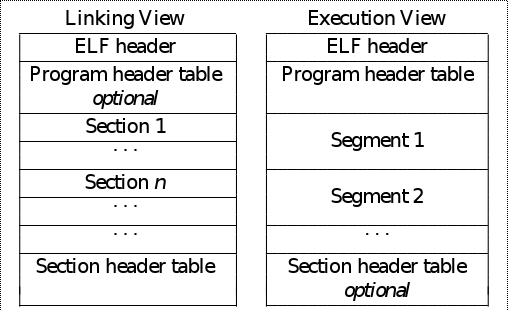
\includegraphics[scale=.4]{./anexo1/images/ELF_Link_exec1} \end{center}
  \caption{Formato ELF}\label{elf1}
\end{figure}

Las secciones pueden almacenar c�digo ejecutable, datos, informaci�n de enlazado din�mico, datos de depuraci�n, tablas de s�mbolos,comentarios, tablas de cadenas, y notas. Las secciones m�s importantes son:

\begin{itemize}
 \item \textbf{.bss}            Datos no inicializados. (RAM)
 \item \textbf{.comment}        Informaci�n de la versi�n.
 \item \textbf{.data y .data1}  Datos inicializados.    (RAM)
 \item \textbf{.debug}          Informaci�n para depuraci�n simb�lica. 
 \item \textbf{.dynamic}        Informaci�n sobre enlace din�mico 
 \item \textbf{.dynstr}         Strings necesarios para el enlace din�mico 
 \item \textbf{.dynsym}         Tabla de s�mbolos utilizada para enlace din�mico.
 \item \textbf{.fini}           C�digo de terminaci�n de proceso.
 \item \textbf{.init}           C�digo de inicializaci�n de proceso.
 \item \textbf{.line}           Informaci�n de n�mero de l�nea para depuraci�n simb�lica.
 \item \textbf{.rodata y .rodta1} Datos de solo-lectura (ROM)
 \item \textbf{.shstrtab}       Nombres de secciones.
 \item \textbf{.symtab}         Tabla de s�mbolos.
 \item \textbf{.text}           Instrucciones ejecutables (ROM)
\end{itemize}

%Falta explicar los ELF dinamicos usados en linux y un ejemplo de como la memoria virtual usa estos archivos

%% Ejemplo de aplicaci�n
Para aclarar el contenido de cada una de estas secciones, consideremos la siguiente aplicaci�n sencilla:

\begin{lstlisting}
#include <stdio.h>

int global;
int global_1 = 1;

int main(void)
{
  int i;                                // Variable no inicializada
  int j = 2;                            // Variable inicializada
  for(i=0; i<10; i++){
    printf("Printing %d\n", i*j);       // Caracteres constantes
    j = j + 1;
    global   = i;
    global_1 = i+j;
  }
  return 0;
}
\end{lstlisting}

Generemos el objeto compil�ndolo con el siguiente comando:
\textit{arm-none-linux-gnueabi-gcc -c hello.c}

Examinemos que tipo de secciones tiene este ejecutable
\textit{arm-none-linux-gnueabi-readelf -S hello.o}

\begin{lstlisting}[style=numbered]
Section Headers:
  [Nr] Name              Type            Addr     Off    Size   ES Flg Lk Inf Al
  [ 0]                   NULL            00000000 000000 000000 00      0   0  0
  [ 1] .text             PROGBITS        00000000 000034 00009c 00  AX  0   0  4
  [ 2] .rel.text         REL             00000000 000484 000020 08      9   1  4
  [ 3] .data             PROGBITS        00000000 0000d0 000004 00  WA  0   0  4
  [ 4] .bss              NOBITS          00000000 0000d4 000000 00  WA  0   0  1
  [ 5] .rodata           PROGBITS        00000000 0000d4 000010 00   A  0   0  4
  [ 6] .comment          PROGBITS        00000000 0000e4 00004d 00      0   0  1
  [ 7] .ARM.attributes   ARM_ATTRIBUTES  00000000 000131 00002e 00      0   0  1
  [ 8] .shstrtab         STRTAB          00000000 00015f 000051 00      0   0  1
  [ 9] .symtab           SYMTAB          00000000 000368 0000f0 10     10  11  4
  [10] .strtab           STRTAB          00000000 000458 00002b 00      0   0  1
Key to Flags:
  W (write), A (alloc), X (execute), M (merge), S (strings)
  I (info), L (link order), G (group), x (unknown)
  O (extra OS processing required) o (OS specific), p (processor specific)
\end{lstlisting}

La secci�n \textit{.text}, como se dijo anteriormente contiene las instrucciones ejecutables, por esta raz�n se marca como ejecutable \textit{``X''} en la columna \textit{Flg}. Es posible ver las instrucciones que se ejecutan en esta secci�n ejecutando:

\textit{arm-none-linux-gnueabi-objdump -d -j .text hello.o}

\begin{lstlisting}[style=numbered]
00000000 <main>:
   0:   e92d4800        stmdb   sp!, {fp, lr}
   4:   e28db004        add     fp, sp, #4      ; 0x4
   8:   e24dd008        sub     sp, sp, #8      ; 0x8
   c:   e3a03002        mov     r3, #2  ; 0x2
  10:   e50b3008        str     r3, [fp, #-8]
  14:   e3a03000        mov     r3, #0  ; 0x0
  18:   e50b300c        str     r3, [fp, #-12]
  1c:   ea000013        b       70 <main+0x70>
  20:   e51b200c        ldr     r2, [fp, #-12]
  24:   e51b3008        ldr     r3, [fp, #-8]
  28:   e0030392        mul     r3, r2, r3
  2c:   e59f005c        ldr     r0, [pc, #92]   ; 90 <.text+0x90>
  30:   e1a01003        mov     r1, r3
  34:   ebfffffe        bl      0 <printf>
  38:   e51b3008        ldr     r3, [fp, #-8]
  3c:   e2833001        add     r3, r3, #1      ; 0x1
  40:   e50b3008        str     r3, [fp, #-8]
  44:   e59f2048        ldr     r2, [pc, #72]   ; 94 <.text+0x94>
  48:   e51b300c        ldr     r3, [fp, #-12]
  4c:   e5823000        str     r3, [r2]
  50:   e51b200c        ldr     r2, [fp, #-12]
  54:   e51b3008        ldr     r3, [fp, #-8]
  58:   e0822003        add     r2, r2, r3
  5c:   e59f3034        ldr     r3, [pc, #52]   ; 98 <.text+0x98>
  60:   e5832000        str     r2, [r3]
  64:   e51b300c        ldr     r3, [fp, #-12]
  68:   e2833001        add     r3, r3, #1      ; 0x1
  6c:   e50b300c        str     r3, [fp, #-12]
  70:   e51b300c        ldr     r3, [fp, #-12]
  74:   e3530009        cmp     r3, #9  ; 0x9
  78:   daffffe8        ble     20 <main+0x20>
  7c:   e3a03000        mov     r3, #0  ; 0x0
  80:   e1a00003        mov     r0, r3
  84:   e24bd004        sub     sp, fp, #4      ; 0x4
  88:   e8bd4800        ldmia   sp!, {fp, lr}
  8c:   e12fff1e        bx      lr
\end{lstlisting}

La secci�n \textit{.data} mantiene las variables inicializadas, y contiene:
 
\textit{arm-none-linux-gnueabi-objdump -d -j .data hello.o}
 
\begin{lstlisting}[style=numbered]
00000000 <global_1>:
   0:   01 00 00 00
\end{lstlisting}

Como vemos, la secci�n \textit{.data} contiene �nicamente el valor de inicializaci�n de la variable \textit{global\_1} (1) y no muestra informaci�n acerca de la variable \textit{j}, esto se debe a que la informaci�n est� en el \textit{stack} del proceso. Si observamos el contenido de la secci�n \textit{.text} observamos que esta variable es asignada en tiempo de ejecuci�n, en la l�nea \textit{0c:} se ve la asignaci�n de esta variable:

\begin{lstlisting}[style=numbered]
0c:   e3a03002        mov     r3, #2  ; 0x2 
10:   e50b3008        str     r3, [fp, #-8]
\end{lstlisting}

La secci�n \textit{.bss} mantiene la informaci�n de las variables no inicializadas. En Linux todas las variables no inicializadas, se inicializaran en cero:

\textit{arm-none-linux-gnueabi-objdump -d -j .bss hello}
 
\begin{lstlisting}[style=numbered]
000145c4 <global>:
    145c4:       00000000
\end{lstlisting}
   
La secci�n \textit{.rodata} contiene los datos que no cambian durante la ejecuci�n del programa, es decir, los de solo lectura, si examinamos esta secci�n obtenemos:
 
\textit{hexdump -C hello.o | grep -i 000000d0} (la secci�n \textit{.rodata} comienza en la posici�n de memoria 0xd4)
 
  
\begin{lstlisting}[style=numbered]
000000d0  01 00 00 00 50 72 69 6e  74 69 6e 67 20 25 64 0a  |....Printing %d.|
000000e0  00 00 00 00 00 47 43 43  3a 20 28 43 6f 64 65 53  |.....GCC: (CodeS|
\end{lstlisting}
 
Observamos que en el archivo se almacena la cadena de caracteres \textit{Printing \%d\\n} la cual no se modifica durante la ejecuci�n del programa.
\subsection{Script del enlazador \textit{Linker}}
\subsubsection{Linker Script}
Como vimos anteriormente, el \textit{linker} es el encargado de agrupar todos los archivos objeto \textit{.o}, y las librer�as necesarias para crear el ejecutable, este \textit{linker} permite definir donde ser�n ubicados los diferentes segmentos del archivo ELF, por medio de un archivo de enlace \textit{linker script}. De esta forma podemos ajustar el ejecutable a plataformas con diferentes configuraciones de memoria. Esto brinda un grado mayor de flexibilidad de la cadena de herramientas GNU. Cuando se dispone de un sistema operativo como Linux no es necesario definir este archivo para los ejecutables, ya que el sistema operativo se encarga de guardar las secciones en el lugar indicado; sin embargo, es necesario tenerlo presente ya que como veremos m�s adelante existe un momento en el que el sistema operativo no ha sido cargado en la plataforma y las aplicaciones que se ejecuten deben proporcionar esta informaci�n. A continuaci�n se muestra un ejemplo de este archivo:

\lstset{emph={flash}, emphstyle=\color{red}, emph={[2]ram,base},emphstyle={[2]\color{blue}}}

\begin{lstlisting}
 /* identify the Entry Point  (_vec_reset is defined in file crt.s)  */
ENTRY(_vec_reset)

/* specify the memory areas  */
MEMORY 
{
    flash : ORIGIN = 0,          LENGTH = 256K    /* FLASH EPROM          */
    ram   : ORIGIN = 0x00200000, LENGTH = 64K     /* static RAM area      */
}

/* define a global symbol _stack_end */
_stack_end = 0x20FFFC;

/* now define the output sections  */
SECTIONS
{
  . = 0;            /* set location counter to address zero  */
  .text :           /* collect all sections that should go into FLASH after startup  */
  {
    *(.text)        /* all .text sections (code)  */
    *(.rodata)      /* all .rodata sections (constants, strings, etc.)  */
    *(.rodata*)     /* all .rodata* sections (constants, strings, etc.)  */
    *(.glue_7)      /* all .glue_7 sections  (no idea what these are) */
    *(.glue_7t)     /* all .glue_7t sections (no idea what these are) */
    _etext = .;     /* define a global symbol _etext just after the last code byte */
  } >flash          /* put all the above into FLASH */

  .data :           /* collect all initialized .data sections that go into RAM  */ 
  {
    _data = .;      /* create a global symbol marking the start of the .data section  */
    *(.data)        /* all .data sections  */
    _edata = .;     /* define a global symbol marking the end of the .data section  */
  } >ram AT >flash  /* put all the above into RAM (but load the LMA initializer copy 
                       into FLASH)  */

  .bss :            /* collect all uninitialized .bss sections that go into RAM  */
  {
    _bss_start = .; /* define a global symbol marking the start of the .bss section */
    *(.bss)         /* all .bss sections  */
  } >ram            /* put all the above in RAM (it will be cleared in the startup code*/
  . = ALIGN(4);     /* advance location counter to the next 32-bit boundary */
  _bss_end = . ;    /* define a global symbol marking the end of the .bss section */
}
_end = .;           /* define a global symbol marking the end of application RAM */
\end{lstlisting}

En las primeras l�neas del archivo aparece la declaraci�n de las memorias de la plataforma; en este ejemplo, tenemos una memoria RAM de 64kB que comienza en la posici�n de memoria 0x00200000 y una memoria flash de 256k que comienza en la posici�n 0x0. A continuaci�n se definen las secciones y el lugar donde ser�n almacenadas; en este caso, las secciones \textit{.text} (c�digo ejecutable) y \textit{.rodata} (datos de solo lectura) se almacenan en una memoria no vol�til la flash. Cuando el sistema sea energizado el procesador ejecutar� el c�digo almacenado en su memoria no vol�til. Las secciones \textit{.data} (variables inicializadas) y \textit{.bss} (variables no inicializadas) se almacenar�n en la memoria vol�til RAM, ya que el acceso a las memorias no vol�tiles son m�s lentas y tienen ciclos de lectura/escritura finitos.

En algunos SoCs no se dispone de una memoria no vol�til, por lo que es necesario que la aplicaci�n sea cargada por completo en la RAM. Algunos desarrolladores prefieren almacenar y ejecutar sus aplicaciones en las memorias vol�tiles durante la etapa de desarrollo, debido a que la programaci�n de las memorias no vol�tiles toman mucho m�s tiempo. Obviamente una vez finalizada la etapa de desarrollo las aplicaciones deben ser almacenadas en memorias no vol�tiles.


%%%%%%%%%%%%%%%%%%%%% %%%%%%%%%%% %%%%%%%%%%%%%%%%%%%%%%%%%%%%%%%%%
%
% This section is intended to provide a review on how to use the 
% GNU Toolchain and its parts to buil SW
%
%%%%%%%%%%%%%%%%%%%%%%%% %%%%%%%%%%%%%%% %%%%%%%%%%%%%%%%%%%%%%%%%%
\section{Herramientas libres para simulaci�n dise�o de Hardware por descripci�n de hardware}


\subsubsection{S�ntesis, simulaci�n y verificaci�n digital}

Para la s�ntesis digital a partir de lenguajes de descripci�n de hardware se utilizan las herramientas gratuitas suministradas por los fabricantes de FPGAs, \textit{webpack} de Xilinx y \textit{Quartus} de Altera; debido a que la estructura interna de las FPGAs solo la conocen los fabricantes\footnote{Es posible obtener informaci�n valiosa de sus patentes por ejemplo: http://www.freepatentsonline.com/6301693.pdf, con este tipo de informaci�n varios proyectos buscan generar herramientas abiertas de s�ntesis}, es obligatorio utilizar sus herramientas para obtener el archivo de configuraci�n.

Para la simulaci�n de sistemas digitales que utilizan como entrada de dise�o lenguajes de descripci�n de hardware existen los simuladores \textit{ICARUS} para verilog y \textit{GHDL} para vhdl; los dos pueden ser utilizados para realizar simulaciones funcionales, post s�ntesis o post place \& route (trabajando en conjunto con las herramientas de los fabricantes) y ambos soportan el formato de salida VCD (definido junto con el lenguaje de descripci�n de hardware verilog por el est�ndar IEEE 1364-2001). Adicionalmente, estas herramientas pueden ser utilizadas en los sistemas operativos m�s utilizados.

Como herramienta de simulaci�n se utilizar� \textit{GTKWAVE}, la cual acepta como entrada archivos en formato \textit{VCD} y puede ser ejecutada en MAC, Linux y Windows. \textit{GTKWAVE} realiza un manejo adecuado de la jerarqu�a del sistema bajo an�lisis, permitiendo observar todas las se�ales de los diferentes m�dulos que componen la jerarqu�a superior, lo que es muy �til en este tipo de simulaciones; en la figura \ref{gtkwave} se puede observar una captura de esta herramienta.

  \begin{figure}[htpb]
    \begin{center} 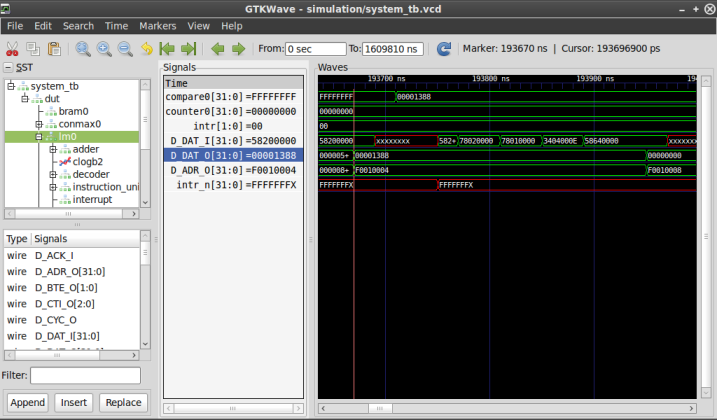
\includegraphics[scale=.7]{./anexo1/images/gtkwave.png}   \end{center}
     \caption{Visualizador de formas de onda \textit{GTKWAVE}} \label{gtkwave}
  \end{figure}

Una vez configurada la FPGA, se utiliza la herramienta \textit{URJTAG} para verificar el correcto funcionamiento del sistema implementado en la FPGA, \textit{URJTAG} proporciona una capa de abstracci�n de hardware que permite el manejo del puerto JTAG de cualquier dispositivo, proporcionando funciones de alto nivel para la aplicaci�n de las funciones JTAG (IDCODE, INTEST, EXTEST, BYPASS, SAMPLE/PRELOAD) permitiendo la aplicaci�n de vectores de prueba al n�cleo l�gico de la FPGA y la captura de la respuesta a estos est�mulos; estas pruebas se realizan a baja frecuencia. \textit{URJTAG} soporta varias interfaces f�sicas para control de las se�ales del puerto JTAG (TDI, TDO, TMS y TCK) las cuales pueden ser conectadas a diferentes puertos de un computador, o como en este caso a un puerto virtual creado en el procesador MIPS.  


\subsubsection{Herramientas para la configuraci�n de PLDs}
Aunque con la plataforma de desarrollo SIE no es necesario utilizar herramientas ni unidades de programaci�n adicionales para configurar su FPGA; el procesador de SIE ejecuta dos aplicaciones que son utilizadas para realizar esta funci�n y pueden ser ejecutadas en computadores personales: \textit{URJTAG} y \textit{XC3SPROG}, las dos funcionan de forma similar, utilizan dispositivos conectados al puerto paralelo (conexi�n directa) o USB (basados en el protocolo MPSSE del chip FT2232) del computador; para ejecutar las instrucciones extendidas de la FPGA CFG\_OUT, CFG\_IN, JSTART y JPROGRAM (hasta el momento solo han sido probadas con las FPGAs de Xilinx).



%%%%%%%%%%%%%%%%%%%%% %%%%%%%%%%% %%%%%%%%%%%%%%%%%%%%%%%%%%%%%%%%%
%
% This section is intended to provide a review on how to use the 
% Programming interfaces
%
%%%%%%%%%%%%%%%%%%%%%%%% %%%%%%%%%%%%%%% %%%%%%%%%%%%%%%%%%%%%%%%%%

\subsection{Interfaz JTAG}
A mediados de los 70s, la estructura de pruebas para tarjetas de circuito impreso (PCB, Printed Circuit Boards) se basaba en el uso de la t�cnica ``bed-of-nails''. Este m�todo utilizaba un dispositivo que conten�a una gran cantidad de puntos de prueba, que permit�an el acceso a dispositivos en la tarjeta a trav�s de puntos colocados en la capa de cobre para dicho fin. Las pruebas se realizaban en dos fases: con el circuito apagado y con el circuito funcionando. Con la aparici�n de los dispositivos de montaje superficial se empez� a colocar dispositivos en las dos caras de la tarjeta, y se redujeron de forma considerable las dimensiones de los dispositivos, disminuyendo la distancia f�sica entre las interconexiones (0.4 - 1mm), dificultando el proceso de pruebas tradicional.

A mediados de los 80s un grupo de ingenieros de pruebas miembros de compa��as electr�nicas europeas se reunieron para examinar el problema y buscar posibles soluciones. Este grupo se auto-denomin� JETAG (Joint European Test Action Group). El m�todo de soluci�n propuesto por ellos estaba basado en el concepto de un registro de corrimiento serial colocado alrededor de la frontera dispositivo, de aqu� el nombre ``Boundary Scan''. Despu�s el grupo se asoci� a compa��as norteamericanas y la ``E'' de ``European'' desapareci� del nombre de la organizaci�n convirti�ndose en JTAG (Join Test Action Group).

\subsubsection{Arquitectura BOUNDARY SCAN} 
A cada se�al de entrada o salida se le adiciona un elemento de memoria multi-prop�sito llamado ``Boundary Scan Cell'' (BSC). Las celdas conectadas a los pines de entrada reciben el nombre de ``Celdas de entrada'', y las que est�n conectadas a los pines de salida ``Celdas de salida''. En la Figura \ref{jtag_basics} se muestra esta arquitectura.

\begin{figure}[h]
  \begin{center} 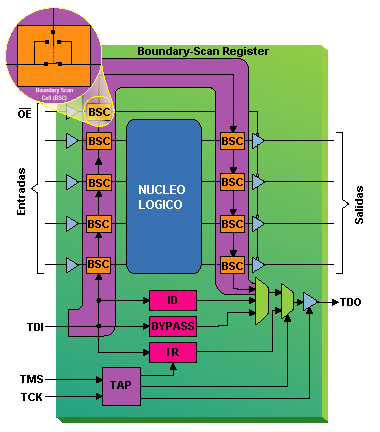
\includegraphics[scale=.6]{./anexo1/images/jtag_basics} \end{center}
  \caption{Arquitectura Boundary Scan} \label{jtag_basics}
\end{figure}

Las BSC se configuran en un registro de corrimiento de entrada y salida paralela. Una carga paralela de los registros (captura) ocasiona que los valores de las se�ales aplicadas a los pines del dispositivo pasen a las celdas de entrada y que opcionalmente los valores de las se�ales internas del dispositivo pasen a las celdas de salida. Una descarga paralela (Actualizaci�n) ocasiona que los valores presentes en las celdas de salida pasen a los pines del dispositivo, y opcionalmente los valores almacenados en las celdas de entrada pasen al interior del dispositivo.

Los datos pueden ser corridos a trav�s del registro de corrimiento de forma serial, empezando por un pin dedicado TDI (Test Data In) y terminando en un pin de salida dedicado llamado TDO (Test Data Out). La se�al de reloj se proporciona por un pin externo TCLK (Test Clock) y el modo de operaci�n se controla por la se�al TMS (Test Mode Select). Los elementos del Boundary Scan no afectan el funcionamiento del dispositivo. Y son independientes del n�cleo l�gico del mismo.

\subsubsection{Instrucciones JTAG}
El Standard IEEE 1149.1 describe tres instrucciones obligatorias: Bypass, Sample/Preload, y Extest \cite{TI96}.

\begin{itemize}
  \item \textbf{BYPASS} Esta instrucci�n permite que el chip permanezca en un modo funcional, hace que el registro de Bypass se coloque entre TDI y TDO; permitiendo la transferencia serial de datos a trav�s del circuito integrado desde TDI hacia TDO sin afectar la operaci�n. La codificaci�n en binario para esta instrucci�n debe ser con todos sus bits en uno. 
  
  \item \textbf{SAMPLE/PRELOAD} Esta instrucci�n selecciona coloca el registro Boundary-Scan entre los terminales TDI y TDO. Durante esta instrucci�n, se puede acceder al registro Boundary-Scan y obtener una muestra de los datos de entrada y salida del chip a trav�s de la operaci�n \textit{Data Scan}. Esta instrucci�n tambi�n se utiliza para precargar los datos de prueba en el registro Boundary-Scan, antes de ejecutar la instrucci�n EXTEST. La codificaci�n de esta instrucci�n la define el fabricante.

  \item \textbf{EXTEST} Esta instrucci�n coloca al circuito integrado en modo de test externo (pruebas de interconexi�n) y conecta el regsitro Boundary-Scan entre TDI y TDO. Las se�ales que salen del circuito son cargadas en el registro boundary-scan en el flanco de bajada de TCK del estado Capture-DR; las se�ales de entrada al dispositivo son cargadas al registro boundary-scan durante el flanco de bajada de TCK dl estado Update-DR (ver Figura \ref{jtag_sm}). La codificaci�n para esta instrucci�n est� definida con todos sus bits en cero.
  
  \item \textbf{INTEST}  La instrucci�n INTEST (opcional) selecciona el registro boundary-scan, pero es utilizado para capturar las se�ales que salen del n�cleo l�gico del dispositivo, y para aplicar valores conocidos a las se�ales de entrada del n�cleo. La codificaci�n para esta se�al es asignada por el dise�ador.
\end{itemize}

\begin{figure}[h]
  \begin{center} 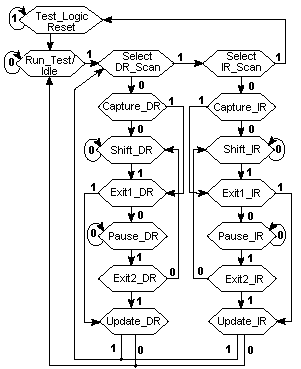
\includegraphics[scale=.8]{./anexo1/images/jtag_sm} \end{center}
  \caption{Arquitectura Boundary Scan} \label{jtag_sm}
\end{figure}



\section{Glosario}
ELF
Objetos
fuentes

binarios
target
reglas
prerequisitos
hdl
codise�o
GNU
GPL
licencias

\section{bib}
No olvidar colocar
Manual del Make tomado de la pagina de GNU project
Managing Projects with GNU Make
